\documentclass[12pt]{article}

\usepackage{sbc-template}

\usepackage{booktabs}
\usepackage{graphicx}
\usepackage{float}
\usepackage{url}
\usepackage{hyperref}
\usepackage{enumerate}
\usepackage{amsmath,bbm}

\usepackage{siunitx}
\sisetup{output-decimal-marker = {,}}

\usepackage[utf8]{inputenc}
\usepackage[brazil]{babel}

\usepackage[alf]{abntex2cite}

\usepackage{multirow}

%% DEFINIÇÃO DE QUADRO
\usepackage{mdframed}
\usepackage{trivfloat}
\usepackage{blindtext}
\trivfloat{quadro}
\floatstyle{plaintop} %Força posição da legenda para o topo
\restylefloat{quadro} %Força posição da legenda para o topo
\renewcommand{\quadroname}{Quadro}
\renewcommand{\listquadroname}{Lista de quadros} %Forçar texto na lista de quadros

%%%%%%%%%%%%%% Python %%%%%%%%%%%%
\usepackage{textcomp}
\usepackage{listings}
\renewcommand{\lstlistlistingname}{Code Listings}
\renewcommand{\lstlistingname}{Code Listing}
\definecolor{gray}{gray}{0.5}
\definecolor{key}{rgb}{0,0.5,0}
\lstnewenvironment{python}[1][]{
\lstset{
language=python,
basicstyle=\ttfamily\small,
otherkeywords={1, 2, 3, 4, 5, 6, 7, 8 ,9 , 0, -, =, +, [, ], (, ), \{, \}, :, *, !},
keywordstyle=\color{blue},
stringstyle=\color{red},
showstringspaces=false,
emph={class, pass, in, for, while, if, is, elif, else, not, and, or,
def, print, exec, break, continue, return},
emphstyle=\color{black}\bfseries,
emph={[2]True, False, None, self},
emphstyle=[2]\color{key},
emph={[3]from, import, as},
emphstyle=[3]\color{blue},
upquote=true,
morecomment=[s]{"""}{"""},
commentstyle=\color{gray}\slshape,
framexleftmargin=0mm, framextopmargin=0mm,#1
}}{} 

%%%%%%%%%%%%%%%%%%%%%%%%%%%%%%%%%%

%% Comentários
\usepackage{xcolor}
\definecolor{lightblue}{RGB}{0,191,255}
\setlength{\marginparwidth}{2cm}
\usepackage[textsize=tiny,backgroundcolor=lightblue,linecolor=lightblue]{todonotes}


%%%%%% Subfiguras -- elloa
\usepackage[bf,sf,footnotesize,indent,justification=centering]{caption}
\usepackage[caption=true,font=footnotesize]{subfig}
\captionsetup[subfigure]{justification=centering,labelfont={bf,sf},textfont={bf,sf,footnotesize},singlelinecheck=off,justification=centering}
\captionsetup[figure]{justification=centering,labelfont={bf,sf},textfont={bf,sf,footnotesize},singlelinecheck=off}
\captionsetup[table]{justification=centering,labelfont={bf,sf},textfont={bf,sf,footnotesize},singlelinecheck=off,justification=centering}
%%%%%%%%%%%%%%%%%%%%%%%%%%%%%%%%%%%%%%%%%%


\sloppy

\title{Verificação de Autenticidade de Assinaturas Manuscritas\\ Utilizando Redes Neurais Convolucionais}

\author{Marcos Wenneton Vieira de Araújo\\
Orientadora: Elloá B. Guedes}

\address{Laboratório de Sistemas Inteligentes\\Grupo de Pesquisas em Sistemas Inteligentes\\
Escola Superior de Tecnologia\\
Universidade do Estado do Amazonas\\
Av. Darcy Vargas, 1200, Manaus, AM
  \email{\{mwvda.eng, ebgcosta\}@uea.edu.br}
}



\begin{document}

\maketitle
\pagestyle{plain} %% Não remover, introduz numeração de páginas -- elloa

\section{Introdução} \label{sec:introducao}

\subsection{Objetivos}

O objetivo geral deste trabalho consiste em verificar a autenticidade de assinaturas manuscritas com redes neurais convolucionais. Para alcançar esta meta, alguns objetivos específicos precisam ser consolidados, a citar:

\begin{enumerate}
  \item Realizar a fundamentação teórica acerca dos conceitos das redes neurais convolucionais;
  \item Consolidar uma base de dados representativa de assinaturas;
  \item Descrever o problema considerado como uma tarefa de Aprendizado de Máquina;
  \item Propor, treinar e testar redes neurais convolucionais para a tarefa considerada;
  \item Analisar os resultados obtidos.
\end{enumerate}

\subsection{Justificativa}

%% Pq resolver esse problema é importante

% Análise de documentos históricos

\subsection{Metodologia}

Para alcançar os objetivos propostos no escopo deste trabalho, a condução das atividades a serem realizadas obedecerá à metodologia descrita a seguir:

\begin{enumerate}
  \item Estudo dos conceitos relacionados ao Aprendizado de Máquinas, Redes Neurais Convolucionais e \emph{Deep Learning};
  \item Descrição do problema considerado como uma tarefa de Aprendizado de Máquina;
  \item Consolidação de uma base de dados representativa de assinaturas originais e forjadas;
  \item Levantamento do ferramental tecnológico para implementação das redes neurais convolucionais;
  \item Proposição de modelos de redes neurais convolucionais para o problema considerado, contemplando arquitetura, parâmetros e hiperparâmetros;
  \item Treino das redes propostas para a tarefa de aprendizado considerada;
  \item Teste das redes previamente treinadas com vistas a coleta de métricas de desempenho;
  \item Análise dos resultados e identificação dos modelos mais adequados para o problema considerado;
  \item Escrita da proposta de Trabalho de Conclusão de Curso;
  \item Defesa da proposta de Trabalho de Conclusão de Curso;
  \item Escrita do Trabalho de Conclusão de Curso; e
  \item Defesa do Trabalho de Conclusão de Curso.
\end{enumerate}

\subsection{Cronograma}

Considerando as atividades enumeradas na metodologia, a Tabela \ref{tab:cronograma} sintetiza o cronograma de execução deste trabalho.

\begin{table}
\scalefont{0.8}
\caption{Cronograma de atividades levando em consideração os dez meses (de $02/2019$ a $12/2019$) para a realização do TCC.}
\label{tab:cronograma}

\begin{center}
\begin{small}
\begin{tabular}{p{5cm}cccccccccccc}
  \toprule
  & &  &  & &  & \textbf{2019}  & &  &  &  &  & \\
                                        & \textbf{02} & \textbf{03} & \textbf{04} & \textbf{05} & \textbf{06} & \textbf{07} & \textbf{08} & \textbf{09} & \textbf{10} & \textbf{11} & \textbf{12} \\
  \midrule

  \textbf{Atividade 1}                     &      X      &      X      &      X      &           &             &             &             &             &             &             &             \\
  \textbf{Atividade 2} &             &      X      &            &             &             &             &             &             &             &             &             \\
  \textbf{Atividade 3}         &             &     X        &    X         &            &            &            &            &            &             &             &             \\
  \textbf{Atividade 4}         &             &             &    X         &            &            &            &            &            &             &             &             \\
  \textbf{Atividade 5}         &             &             &             &      X      &       X     &   X         &     X       &            &             &             &             \\
  \textbf{Atividade 6}         &             &             &             &      X      &     X       &     X       &    X        &            &             &             &             \\
  \textbf{Atividade 7}         &             &             &             &            &            &            &      X      &      X      &             &             &             \\
  \textbf{Atividade 8}         &             &             &             &            &            &            &           &            &   X          &      X       &             \\
  \textbf{Atividade 9}          &      X      &      X      &      X      &      X      &      X      &             &             &             &             &             &             \\

  \textbf{Atividade 10}          &             &             &             &             &      X      &             &             &             &             &             &             \\
  \textbf{Atividade 11}    &             &             &             &             &             &      X      &      X      &      X      &      X      &      X      &      X      \\
  \textbf{Atividade 12}     &             &             &             &             &             &             &             &             &             &             &      X      \\
  \bottomrule
\end{tabular}
\end{small}
\end{center}
\end{table}


\subsection{Organização do Documento}

(..)


\section{Fundamentação Teórica} \label{sec:fund-teor}

A fundamentação teórica para a elaboração deste trabalho consiste em conceitos ligados ao \emph{Machine Learning}. Primeiramente, os conceitos gerais desta área serão apresentados na Seção \ref{subsec:ml}, seguidos pelas características das Redes Neurais Artificais na Seção \ref{subsec:rna}. As definições elementares da técnica de \emph{Machine Learning} conhecida como \emph{Deep Learning} são apresentadas na Seção \ref{subsec:dl}. A Seção \ref{subsubsec:cnns} discorre sobre as características das Redes Neurais Convolucionais, prosseguindo até a Seção \ref{subsubsec:arq-cnns} onde são apresentadas algumas de suas arquiteturas canônicas. Por fim, a Seção \ref{subsubsec:transfer} contém informações sobre a técnica conhecida como \emph{Transfer Learning}, um conceito emergente utilizado em aplicações de \emph{Deep Learning}.

%%%%%

\subsection{\emph{Machine Learning}}
\label{subsec:ml}

\emph{Machine Learning} (ML), também conhecido como Aprendizado de Máquina, é o estudo sistemático de algoritmos e sistemas que melhoram seu conhecimento ou desempenho com o uso da experiência \cite{flach}. Em 1959, o pioneiro em jogos de computador Arthur Samuels definiu \emph{Machine Learning} como um ``campo de estudos que dá aos computadores a habilidade de aprender sem serem explicitamente programados'' \cite{simon}. De acordo com Murphy \cite{murphy} , \emph{Machine Learning} pode ser definido como um conjunto de métodos que podem detectar padrões em dados automaticamente e, em seguida, utilizar os padrões detectados para predizer dados futuros, ou para realizar outros tipos de decisão sob algum tipo de incerteza.

O \emph{Machine Learning} é comumente dividido em três tipos principais de aprendizado, chamados de supervisionado, não-supervisionado e semi-supervisionado. No caso dos algoritmos de aprendizado supervisionado, o objetivo é aprender um mapeamento de entradas para saídas, dado um conjunto rotulado de pares de entradas e saídas. No aprendizado não supervisionado, o algoritmo é apresentado somente aos dados de entrada, e o seu propósito é encontrar padrões significativos nos mesmos. Este problema não é bem definido, porque geralmente não é especificado o tipo de padrão que deve ser encontrado nos dados. Além disso, diferentemente do aprendizado supervisionado, não existe nenhuma métrica de erro óbvia para utilizar. O aprendizado semi-supervisionado, por sua vez, normalmente combina uma pequena quantidade de dados rotulados com uma grande quantidade de dados não rotulados para criar um classificador próprio. Em alguns casos, a abordagem de aprendizagem semi-supervisionada pode ser de grande valor prático. \cite{khan}

Como mostrado na Figura \ref{fig:tasks}, utilizar os atributos corretos para construir os modelos certos que conquistam determinadas tarefas é a essência de ML. Atributos podem ser definidos como uma ``linguagem'' que descreve os objetos relevantes no domínio do problema. Tendo a representação característica adequada dos objetos do domínio, normalmente, não é necessário retornar ao objeto em si, e é por isso que os atributos têm um papel importante em ML. A tarefa é uma representação abstrata de um problema que deseja-se resolver levando em consideração os objetos do domínio. Dentre as tarefas de aprendizado supervisionado mais utilizadas estão a tarefa de classificação binária ou multiclasse e a tarefa de regressão. Um modelo, por sua vez, é a saída produzida por dados de treinamento aplicados em determinado algoritmo de ML \cite{flach}.

\begin{figure}[H]
\centering
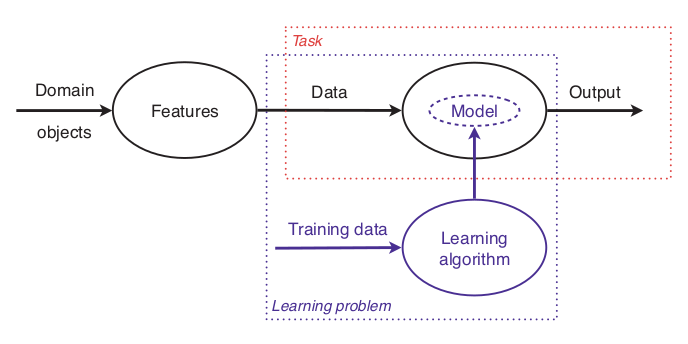
\includegraphics[height=5cm]{imgs/tasks}
\caption{Uma visão geral de como ML é utilizado para adereçar uma tarefa \cite{flach}.}
\label{fig:tasks}
\end{figure}


Em uma tarefa de classificação, um algoritmo é selecionado para especificar quais das $k$ categorias possíveis uma entrada pertence. Para resolver essa tarefa, o algoritmo de aprendizado normalmente produz uma função $f : I\!R^n \rightarrow {1,...,k}$. Quando $y = f(x)$, o modelo denomina uma entrada descrita com o vetor $x$ para uma categoria identificado por um valor numérico $y$ \cite{goodfellow}. Alguns exemplos de tarefa de classificação são a detecção de faces em imagens, a determinação do gênero do indíviduo nessas imagens, a verificação da espécie de uma planta, entre outros.

Quanto à tarefa de regressão, é solicitado a um programa a predição de um valor numérico a partir de uma entrada. Desta forma, o algoritmo de aprendizado é proposto a retornar uma função $f : I\!R^n \rightarrow I\!R$ \cite{goodfellow}. Algumas tarefas de regressão podem ser, por exemplo, a determinação do valor de uma corrida de táxi, a identificação da idade de um indivíduo em uma imagem, prever o preço de uma casa baseado nos dados de casas vendidas anteriormente, etc.

Dentre os tipos de modelos existentes, podemos citar os geométricos, probabilísticos e lógicos. Um modelo geométrico é construído diretamente em função do espaço, utilizando-se de conceitos geométricos como linhas, planos e distâncias. Como exemplos de modelos geométricos temos a regressão linear, o \emph{perceptron} e, em consequência, as redes neurais artificiais. Nos modelos probabilísticos, como o classificador Bayesiano, a questão principal é modelar a relação entre os dados de entrada e saída assumindo que existe algum processo aleatório implícito que produz os valores para essas variáveis, de acordo com uma distribuição de probabilidade bem definida, porém desconhecida. Um modelo lógico, em contrapartida, é o mais naturalmente algorítmico, considerando a capacidade de ser facilmente transformado em regras que podem ser entendidas por seres humanos. Dentre os modelos lógicos estão as árvores de decisão, onde as suas folhas são rotuladas para caracterizar o tipo de tarefa associado ao modelo \cite{flach}.

Dentre os modelos geométricos, as redes neurais artificiais têm demonstrado grande desempenho em diversas áreas. Aplicações de \emph{Deep Learning} para detecção de padrões em imagens e reconhecimento de voz, por exemplo, utilizam-se desses modelos para a obtenção de resultados relevantes. Tomando isto e levando em consideração o contexto deste trabalho, as próximas seções apresentadas abordam significativamente estes conceitos.

%%%%%

\subsection{Redes Neurais Artificiais}
\label{subsec:rna}

As \emph{Redes Neurais Artificiais} (RNAs) são uma tentativa computacional de modelar a capacidade de processamento de informação do cérebro humano \cite{rojas}. Para alcançarem um bom desempenho, as RNAs empregam uma interligação de estruturas bases chamadas de neurônios artificiais que, por sua vez, possuem pesos com valores numéricos positivos ou negativos associados a si. Uma vantagem das RNAS, é a grande capacidade de generalização, ou seja, a habilidade de produzir saídas adequadas para entradas que não estavam presente anteriormente durante sua aprendizagem \cite{haykin}.

A idealização dos neurônios artificiais foi inspirada nos neurônios biológicos encontrados no cérebro humano.

% O \emph{Perceptron} foi desenvolvido em 1957 por Frank Rosenblatt, que mudam com a "experiência", usando uma regra de correção de erros projetada para modificar os pesos de cada unidade de resposta quando faz respostas erradas a estímulos que são apresentados à rede. \cite{arbib}

% \begin{itemize}
% \item Comparação do neuronio artificial com o real;
% \item História e funcionamento do neuronio artificial;
% \item Funções de ativação (talvez depois);
% \item Perceptron (citar o livro do Frank Rosenblatt);
% \item Funcionamento do Perceptron (livro do Marvin Minsky).
% \item Arquiteturas das redes neurais.
% \item Pegar mais escopo do intro to deep learning no Udacity.
% \end{itemize}

\subsubsection{\emph{Multilayer Perceptron}}
\label{subsubsec:mlp}

%%%%%

\subsection{\emph{Deep Learning}}
\label{subsec:dl}

\subsubsection{Redes Neurais Convolucionais}
\label{subsubsec:cnns}

\subsubsection{Arquiteturas canônicas de Redes Neurais Convolucionais}
\label{subsubsec:arq-cnns}

\subsubsection{\emph{Transfer Learning}}
\label{subsubsec:transfer}


\section{Trabalhos Relacionados} \label{sec:trab-rel}

\section{Solução Proposta} \label{sec:sol-prop}


\section{Visão Geral do Conjunto de Dados}
% estatisticas calculadas lá no notebook



\section{Preparação do Conjunto de Dados}

\begin{table}[h!]
	\centering
	\caption{Divisão dos dados}
	\label{tab:divisao-dados}
	%\scalefont{0.77}
	\begin{tabular}{c c c c c}
		\toprule
		\textbf{Abordagem} & \textbf{Tipo de Exemplo} & \textbf{Treino} & \textbf{Validação} & \textbf{Teste}\\
		\midrule
		\multirow{2}{*}{1} & genuíno & 2011 & 299 & 618 \\
     & forjado & 11649 & 1648 & 3237 \\
     \midrule
    \multirow{2}{*}{2} & genuíno & 2011 & 299 & 618   \\
     & forjado & 2024 & 308 & 569 \\
		\bottomrule
	\end{tabular}
\end{table}

\begin{figure}[h!]
  \centering
\caption{Visualização da divisão dos dados}
  \subfloat[Abordagem 1\label{subfig:approach1}]{%
    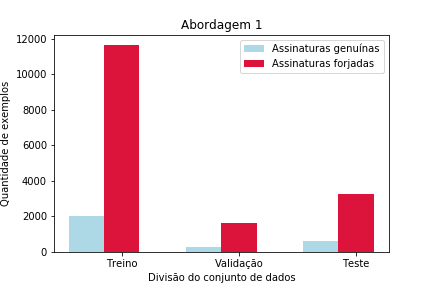
\includegraphics[width=0.7\textwidth]{imgs/approach1}
  }
  \hfill
  \subfloat[Abordagem 2\label{subfig:approach2}]{%
    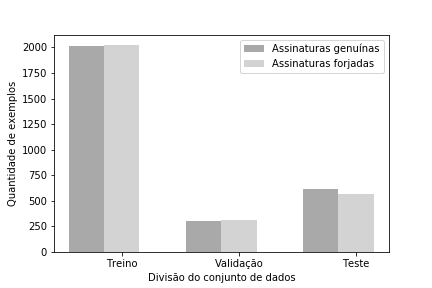
\includegraphics[width=0.7\textwidth]{imgs/approach2}
  }
  \label{fig:divisao-dados}
\end{figure}


\section{Resultados Parciais} \label{sec:res-parc}


\section{Considerações Parciais} \label{sec:cons-parc}





\bibliography{sbc-template}

\end{document}
